% ============================================================
%  Rich picture - PrepMeUp (SW4PRJ4, group 3)
%  Compiles on its own:  pdflatex rich-picture.tex
%  Commit the generated rich-picture.pdf as well (nothing in the
%  report build rebuilds standalone TikZ pictures automatically).
% ============================================================
\documentclass[tikz,border=8pt]{standalone}
\usepackage[T1]{fontenc}
\usepackage[utf8]{inputenc}
\usepackage{lmodern}
\usetikzlibrary{shapes.geometric,arrows.meta,positioning,calc}

\definecolor{deep}{HTML}{173330}
\definecolor{soft}{HTML}{E8F0EE}

\tikzset{
  actor/.style={draw=deep, line width=.6pt, fill=white, rounded corners=3pt,
    text width=30mm, align=center, inner sep=5pt, font=\small},
  system/.style={draw=deep, line width=1pt, fill=soft, rounded corners=4pt,
    text width=40mm, align=center, inner sep=6pt, font=\small\bfseries},
  ext/.style={draw=deep, line width=.6pt, dashed, fill=white, rounded corners=3pt,
    text width=32mm, align=center, inner sep=5pt, font=\small},
  cloud/.style={draw=deep, line width=.6pt, ellipse, fill=white,
    text width=34mm, align=center, inner sep=3pt, font=\small\itshape},
  flow/.style={draw=deep, line width=.6pt, -{Stealth[length=2mm]}},
  lbl/.style={font=\scriptsize, fill=white, inner sep=1.5pt, align=center},
}

\begin{document}
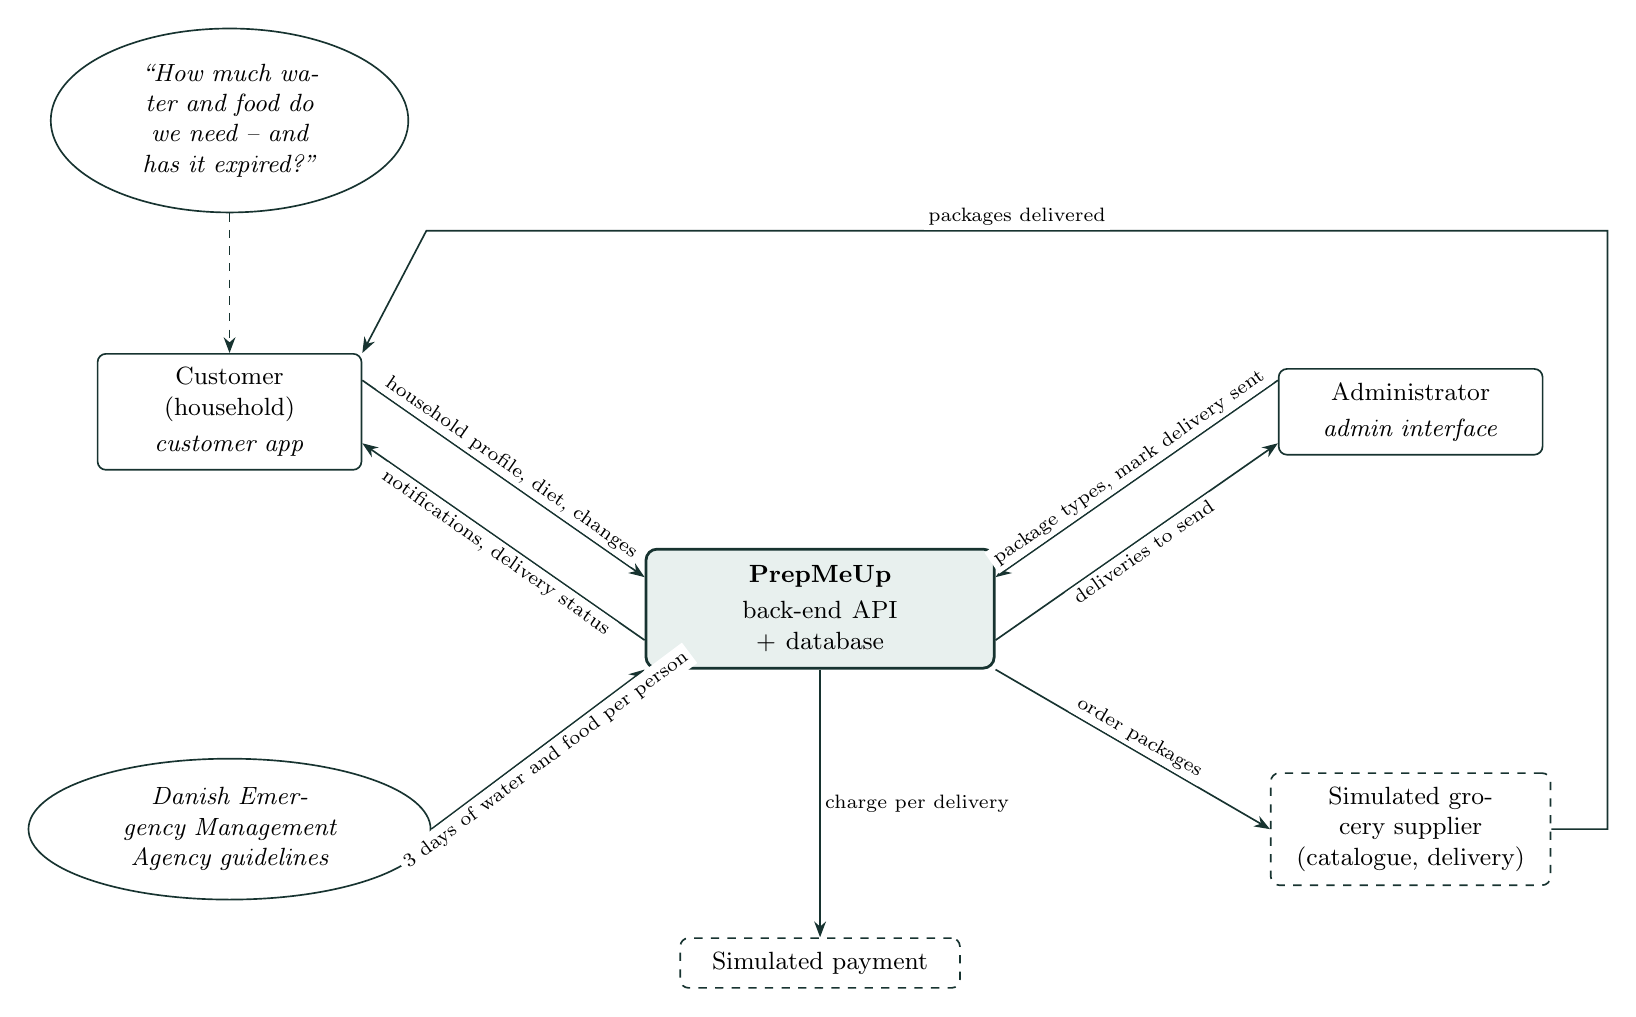
\begin{tikzpicture}[x=1mm,y=1mm]

% ----- central system -----
\node[system] (sys) at (0,0) {PrepMeUp\\[2pt]\normalfont back-end API\\+ database};

% ----- people -----
\node[actor] (customer) at (-75,25) {Customer\\(household)\\[2pt]\emph{customer app}};
\node[actor] (admin) at (75,25) {Administrator\\[2pt]\emph{admin interface}};

% ----- external / simulated -----
\node[ext] (supplier) at (75,-28) {Simulated grocery supplier\\(catalogue, delivery)};
\node[ext] (payment) at (0,-45) {Simulated payment};
\node[cloud] (brs) at (-75,-28) {Danish Emergency Management Agency guidelines};

% ----- concern (thought bubble) -----
\node[cloud, text width=30mm] (worry) at (-75,62) {``How much water and food do we need -- and has it expired?''};

% ----- flows: customer <-> system (two parallel lines) -----
\draw[flow] ([yshift=4mm]customer.east) -- node[lbl,above,sloped]{household profile, diet, changes}
  ([yshift=4mm]sys.west);
\draw[flow] ([yshift=-4mm]sys.west) -- node[lbl,below,sloped]{notifications, delivery status}
  ([yshift=-4mm]customer.east);

% ----- flows: admin <-> system -----
\draw[flow] ([yshift=4mm]admin.west) -- node[lbl,above,sloped]{package types, mark delivery sent}
  ([yshift=4mm]sys.east);
\draw[flow] ([yshift=-4mm]sys.east) -- node[lbl,below,sloped]{deliveries to send}
  ([yshift=-4mm]admin.west);

% ----- flows: inputs and simulated services -----
\draw[flow] (brs.east) -- node[lbl,below,sloped]{3 days of water and food per person} (sys.south west);
\draw[flow] (sys.south) -- node[lbl,right]{charge per delivery} (payment.north);
\draw[flow] (sys.south east) -- node[lbl,above,sloped]{order packages} (supplier.west);

% supplier -> customer: routed around the top so it does not cross the system
\draw[flow] (supplier.east) -- (100,-28) -- (100,48) -- node[lbl,above]{packages delivered} (-50,48) -- (customer.north east);

\draw[flow,dashed] (worry) -- (customer);

\end{tikzpicture}
\end{document}
